\chapter{Results}
\label{chapterlabel6}

A "control simulation" will be defined as the case that is most commonly used in literature. The case used as control will be a normal-sized aorta, smooth wall and Newtonian fluid. The mesh selected was mesh 3 ($\sim$600,000 elements) \cite{Steinman2012AssumptionsHemodynamics}.

\section{Outlet flow and pressure comparison}
A comparison of the outlet conditions was performed. The results were compared by calculating the mean absolute percentage error (MAPE) between control model and the model with modified assumptions:

\begin{align}
    MAPE =| \frac{y_{i}-y_{control}}{y_{control}}| \times 100 \%
\end{align}

where y is the parameter of interest, which in this comparison would be either the flow rate or the pressure. \par
A comparison of the outlet pressure and flow can be seen on the Figures \ref{fig:flow} and \ref{fig:pressure}. A comparison with the control simulation shows that the pressure at the outlets are very similar across the models as the mean absolute percentage error is less then 1\% (as seen in the Table \ref{tab:pererr}). However, significant differences can be seen in the flow curves, depending on the model assumptions taken into account. On the Table \ref{tab:pererr}, very small differences can be seen when the viscosity model is modified while the dilation of the aortic geometry results in a much larger MAPE.
\begin{figure}
     \centering
     \begin{subfigure}[b]{0.49\textwidth}
         \centering
         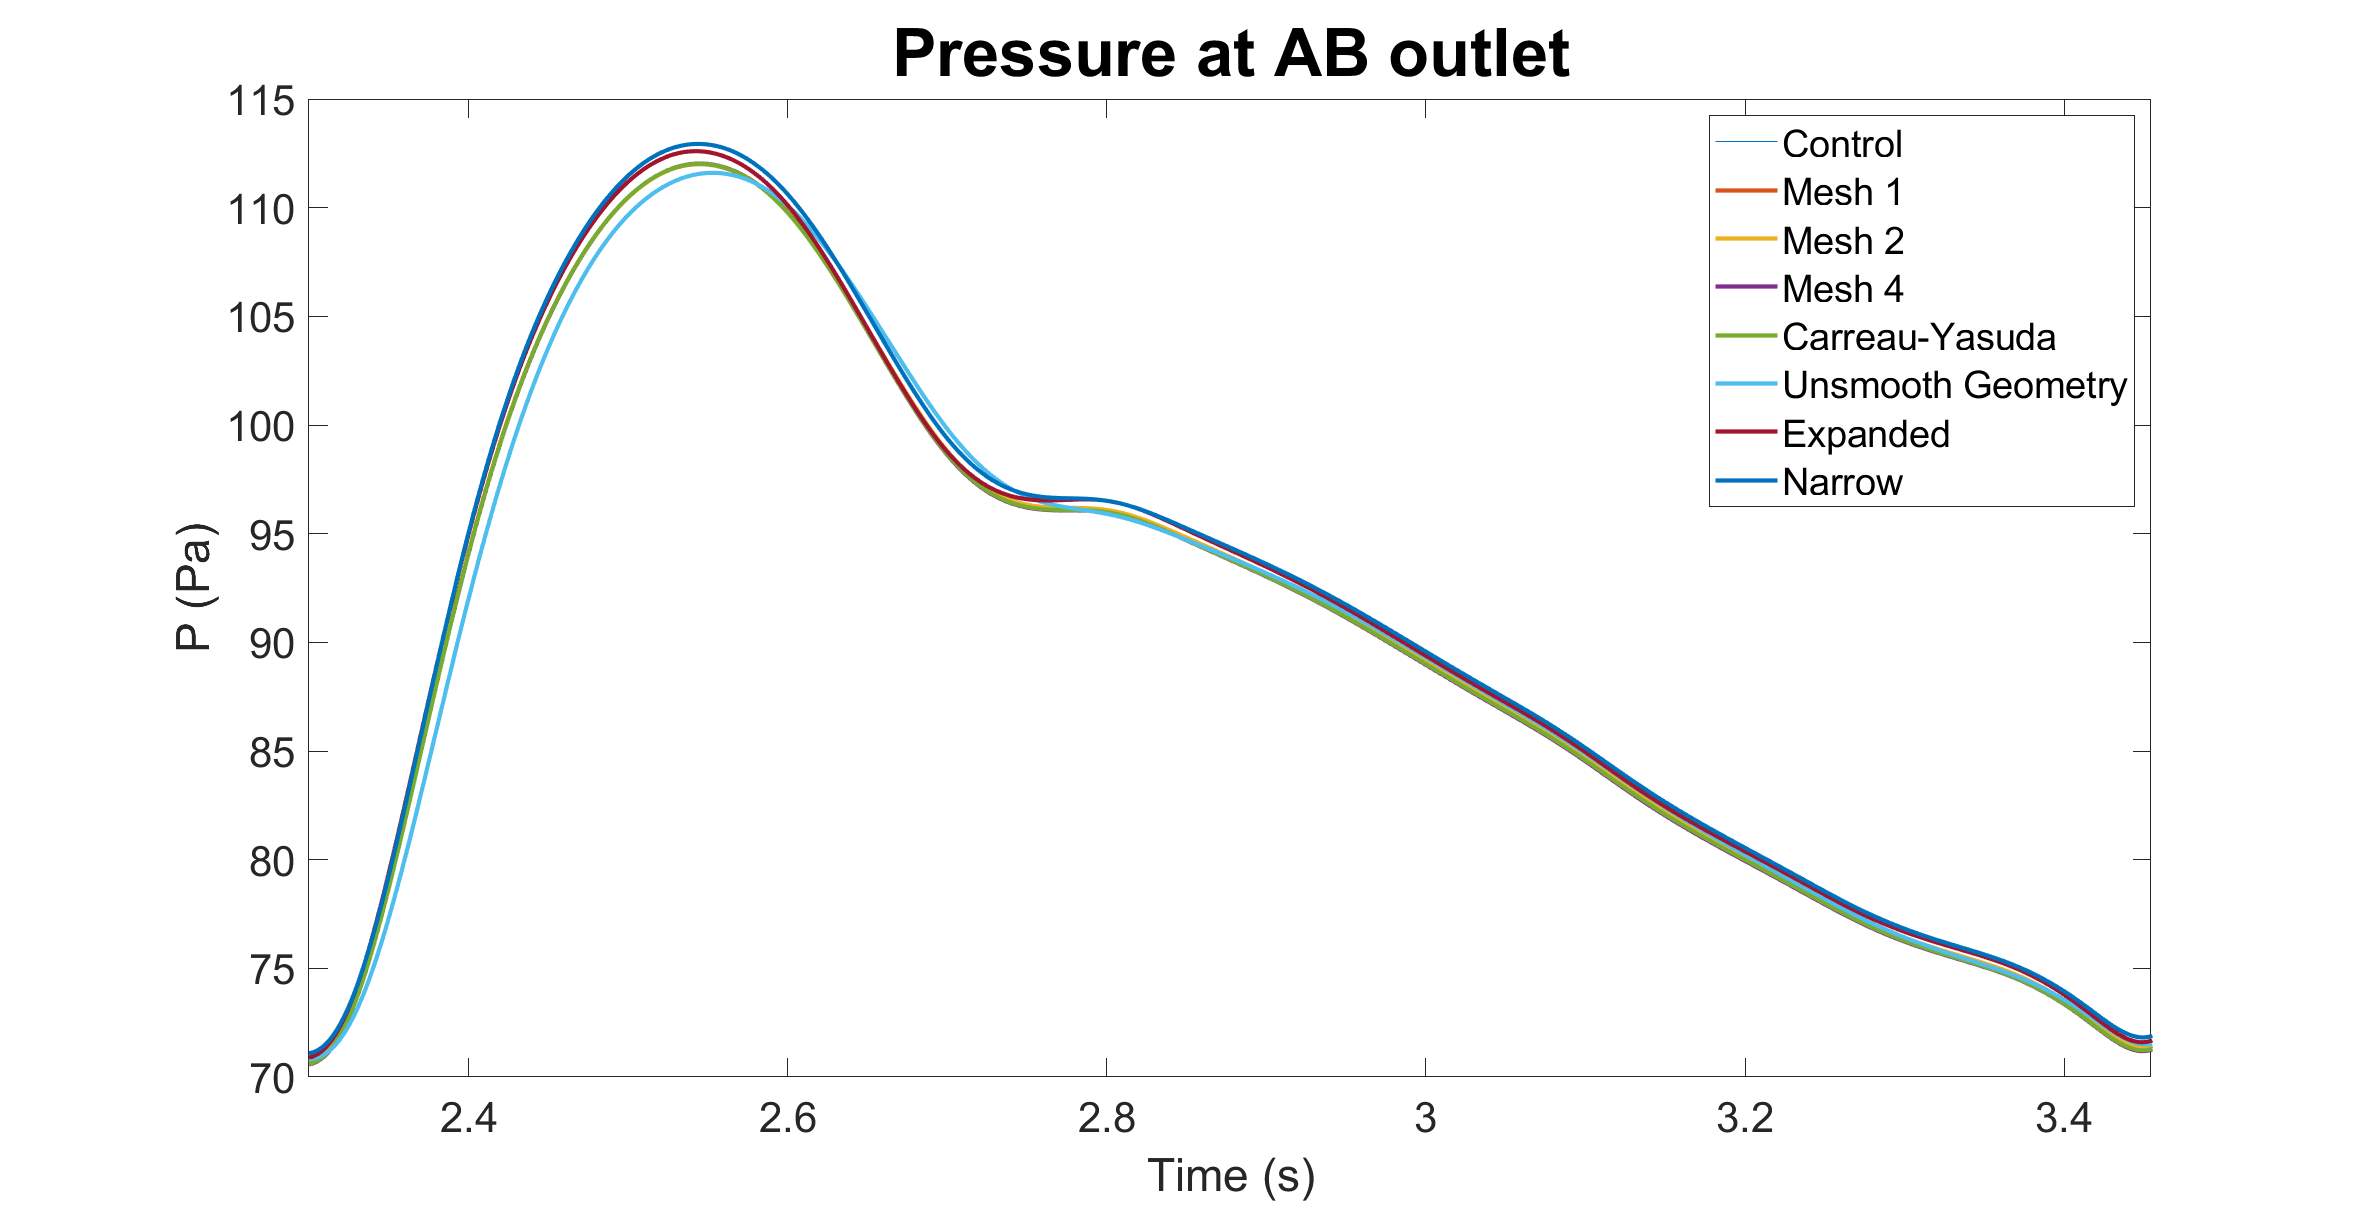
\includegraphics[width=\textwidth]{Figures/PAB.png}
     \end{subfigure}
     \hfill
     \begin{subfigure}[b]{0.49\textwidth}
         \centering
         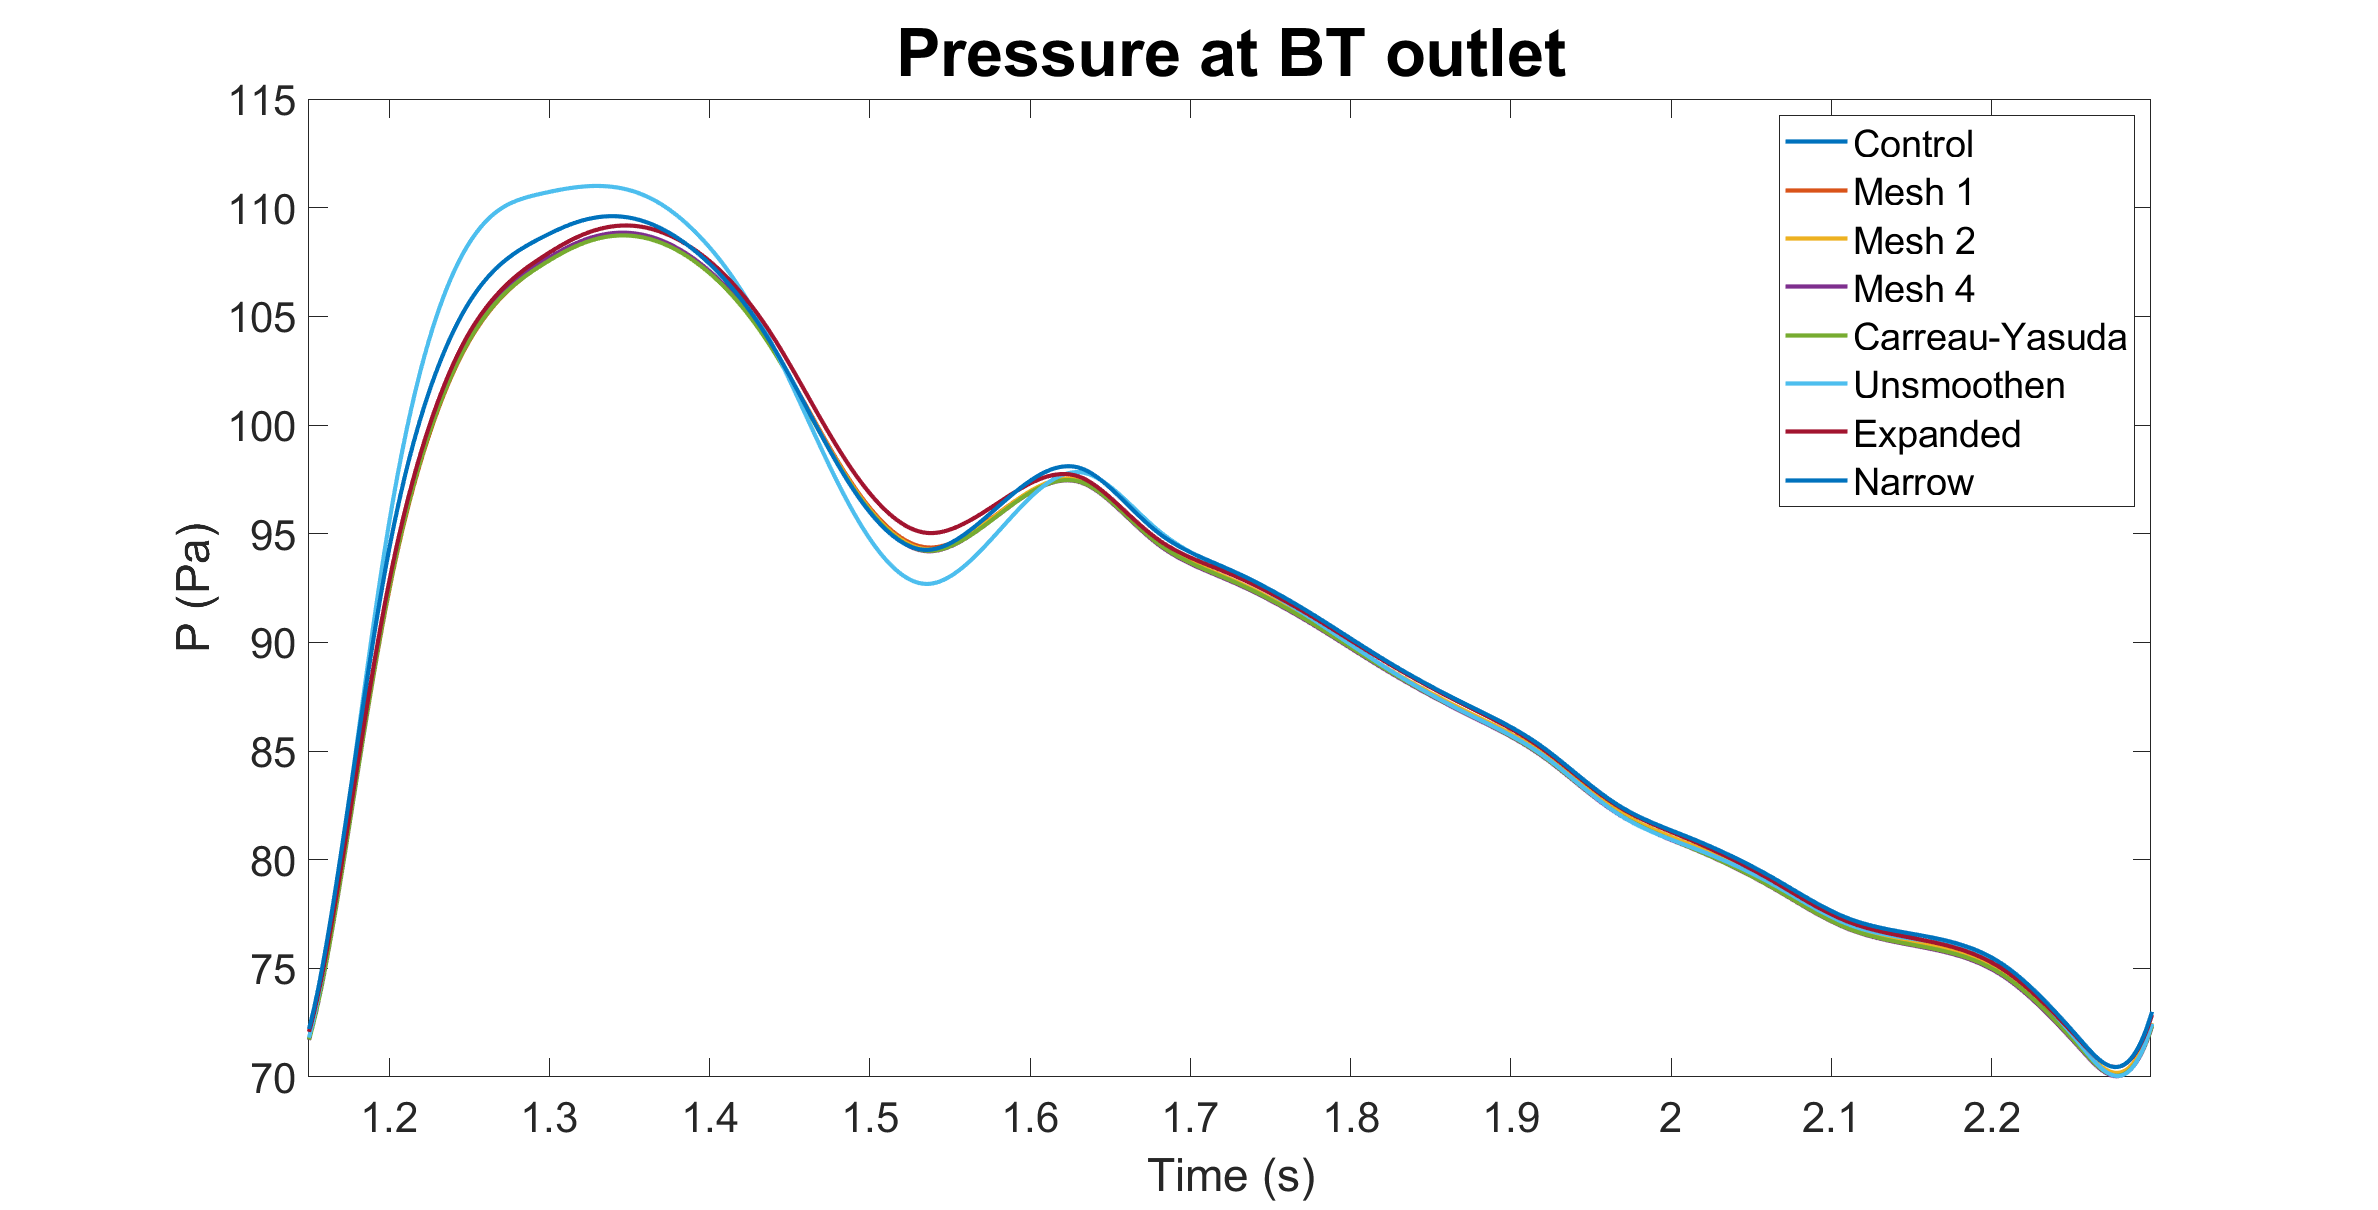
\includegraphics[width=\textwidth]{Figures/PBT.png}
     \end{subfigure}
     \hfill
     \begin{subfigure}[b]{0.49\textwidth}
         \centering
         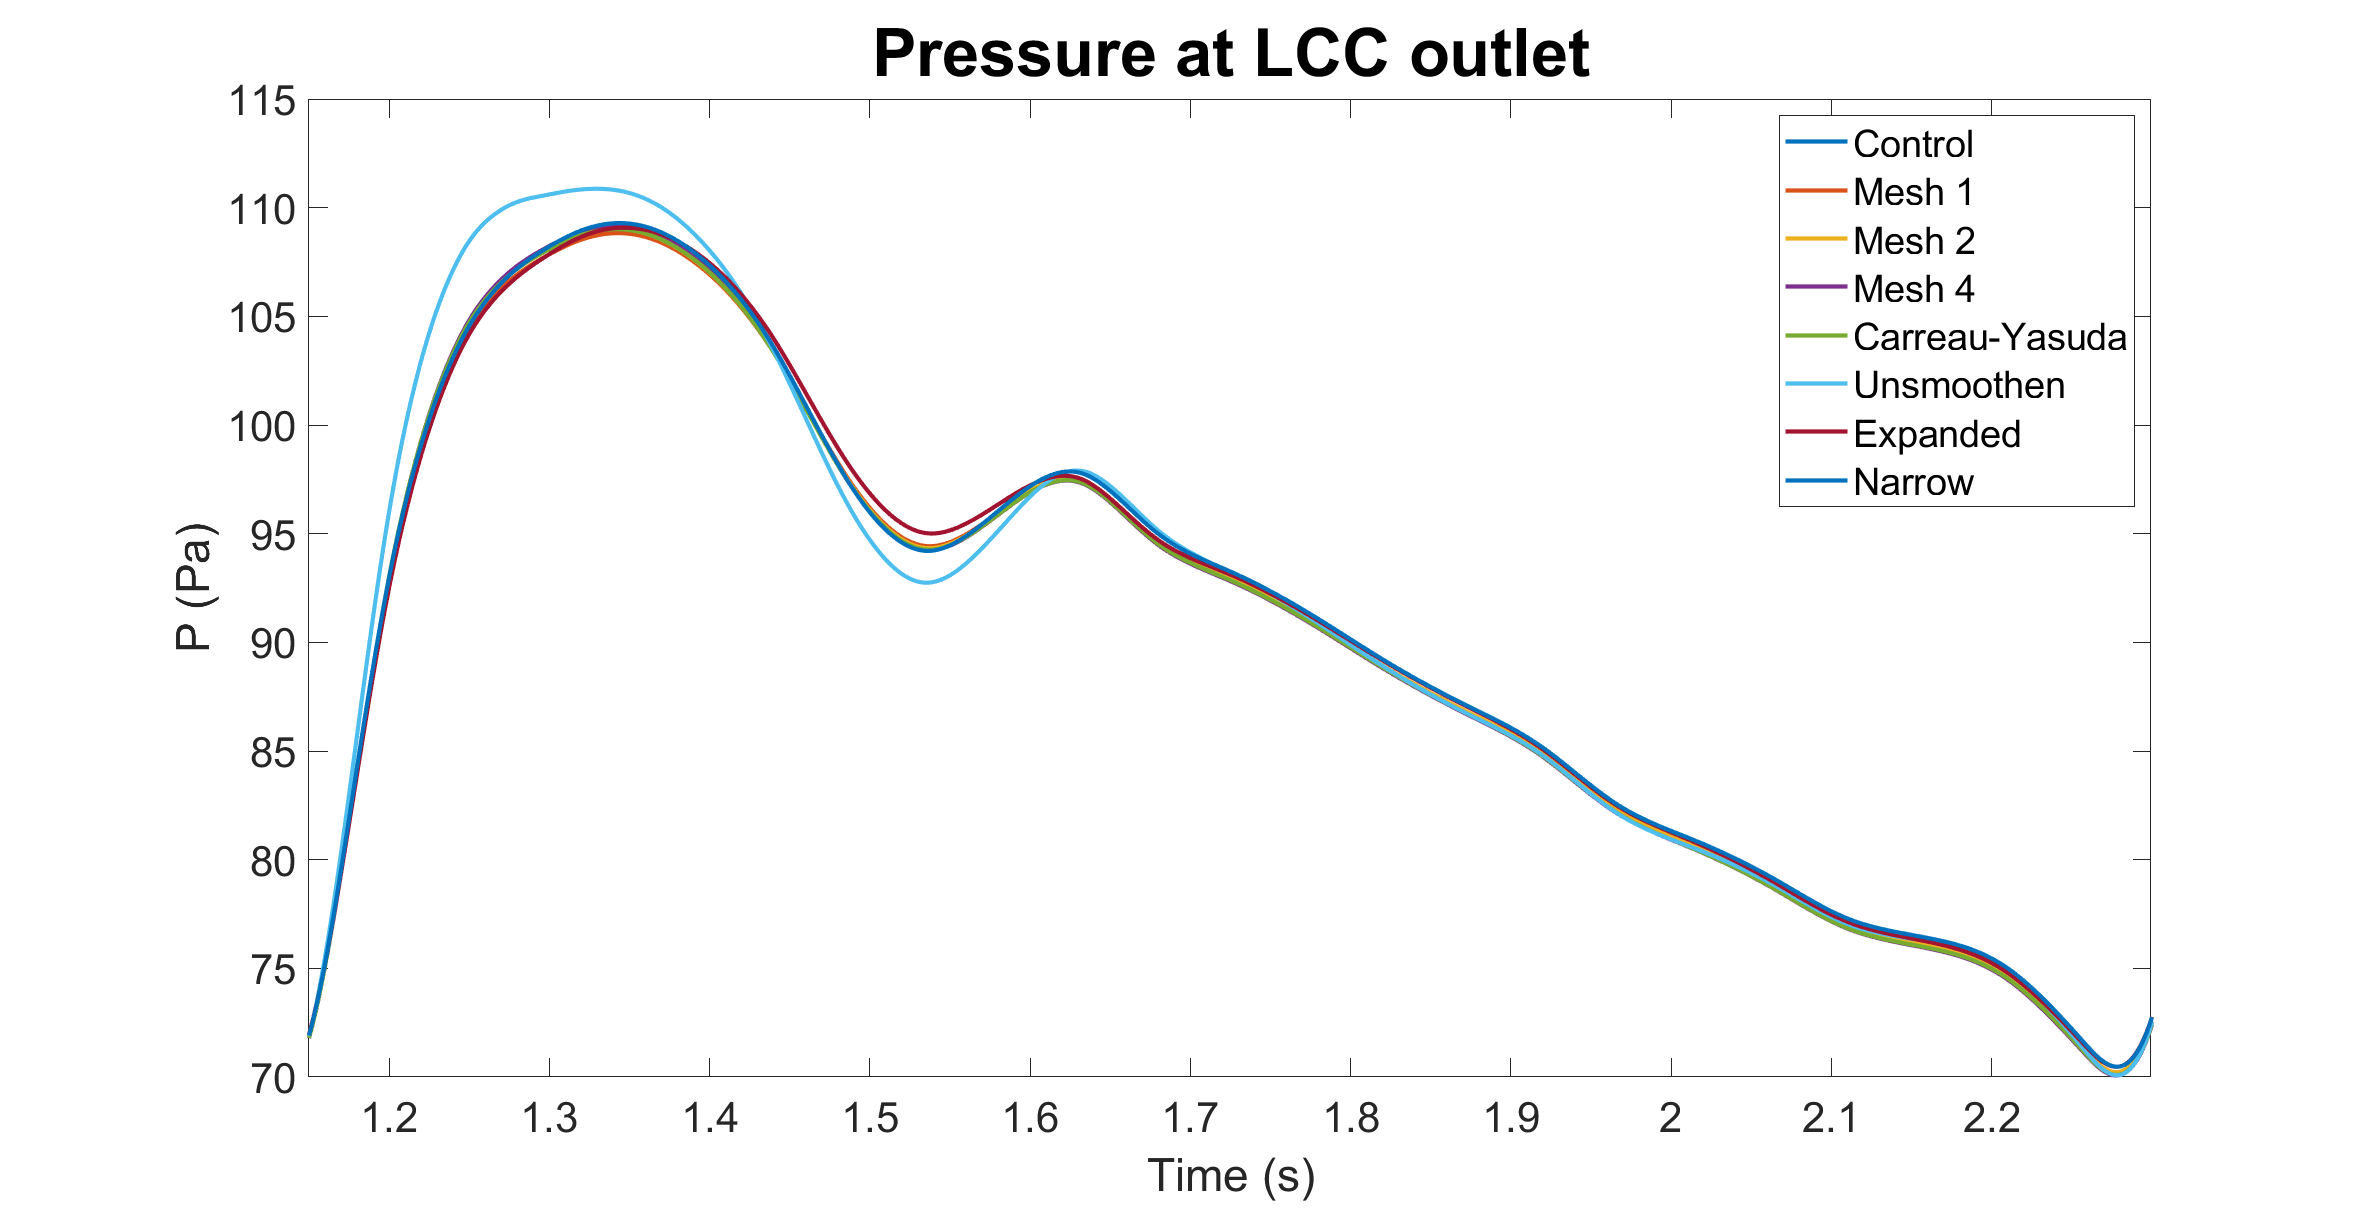
\includegraphics[width=\textwidth]{Figures/PLCC.png}
     \end{subfigure}
     \hfill
     \begin{subfigure}[b]{0.49\textwidth}
         \centering
         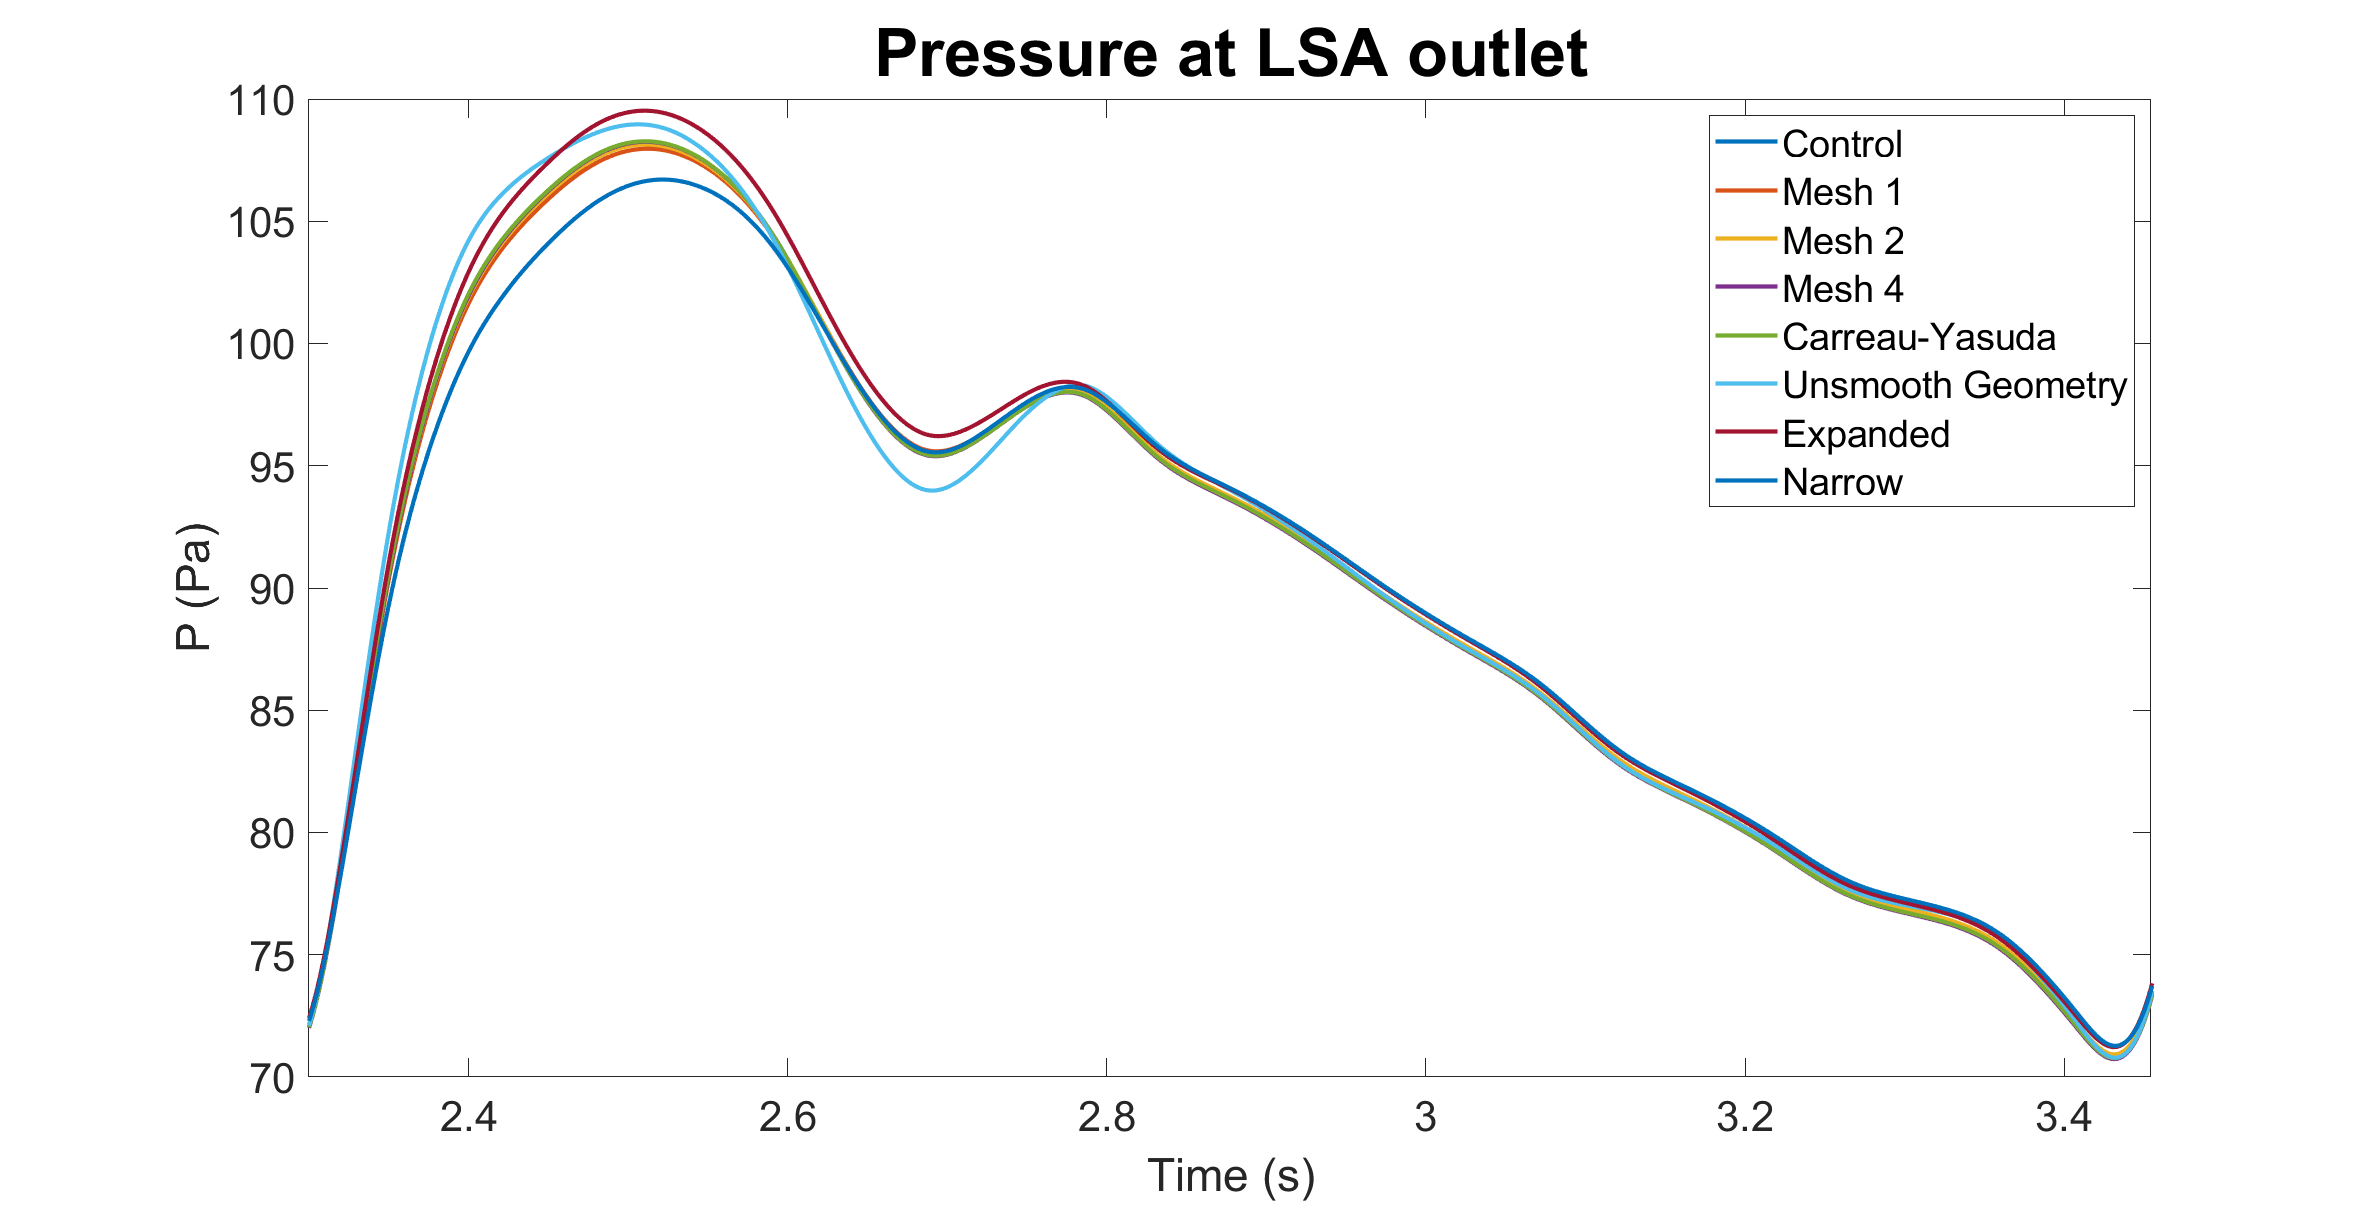
\includegraphics[width=\textwidth]{Figures/PLSA.png}
     \end{subfigure}
        \caption{The pressure at the different outlets}
        \label{fig:pressure}
\end{figure}

\begin{figure}
     \centering
     \begin{subfigure}[b]{0.49\textwidth}
         \centering
         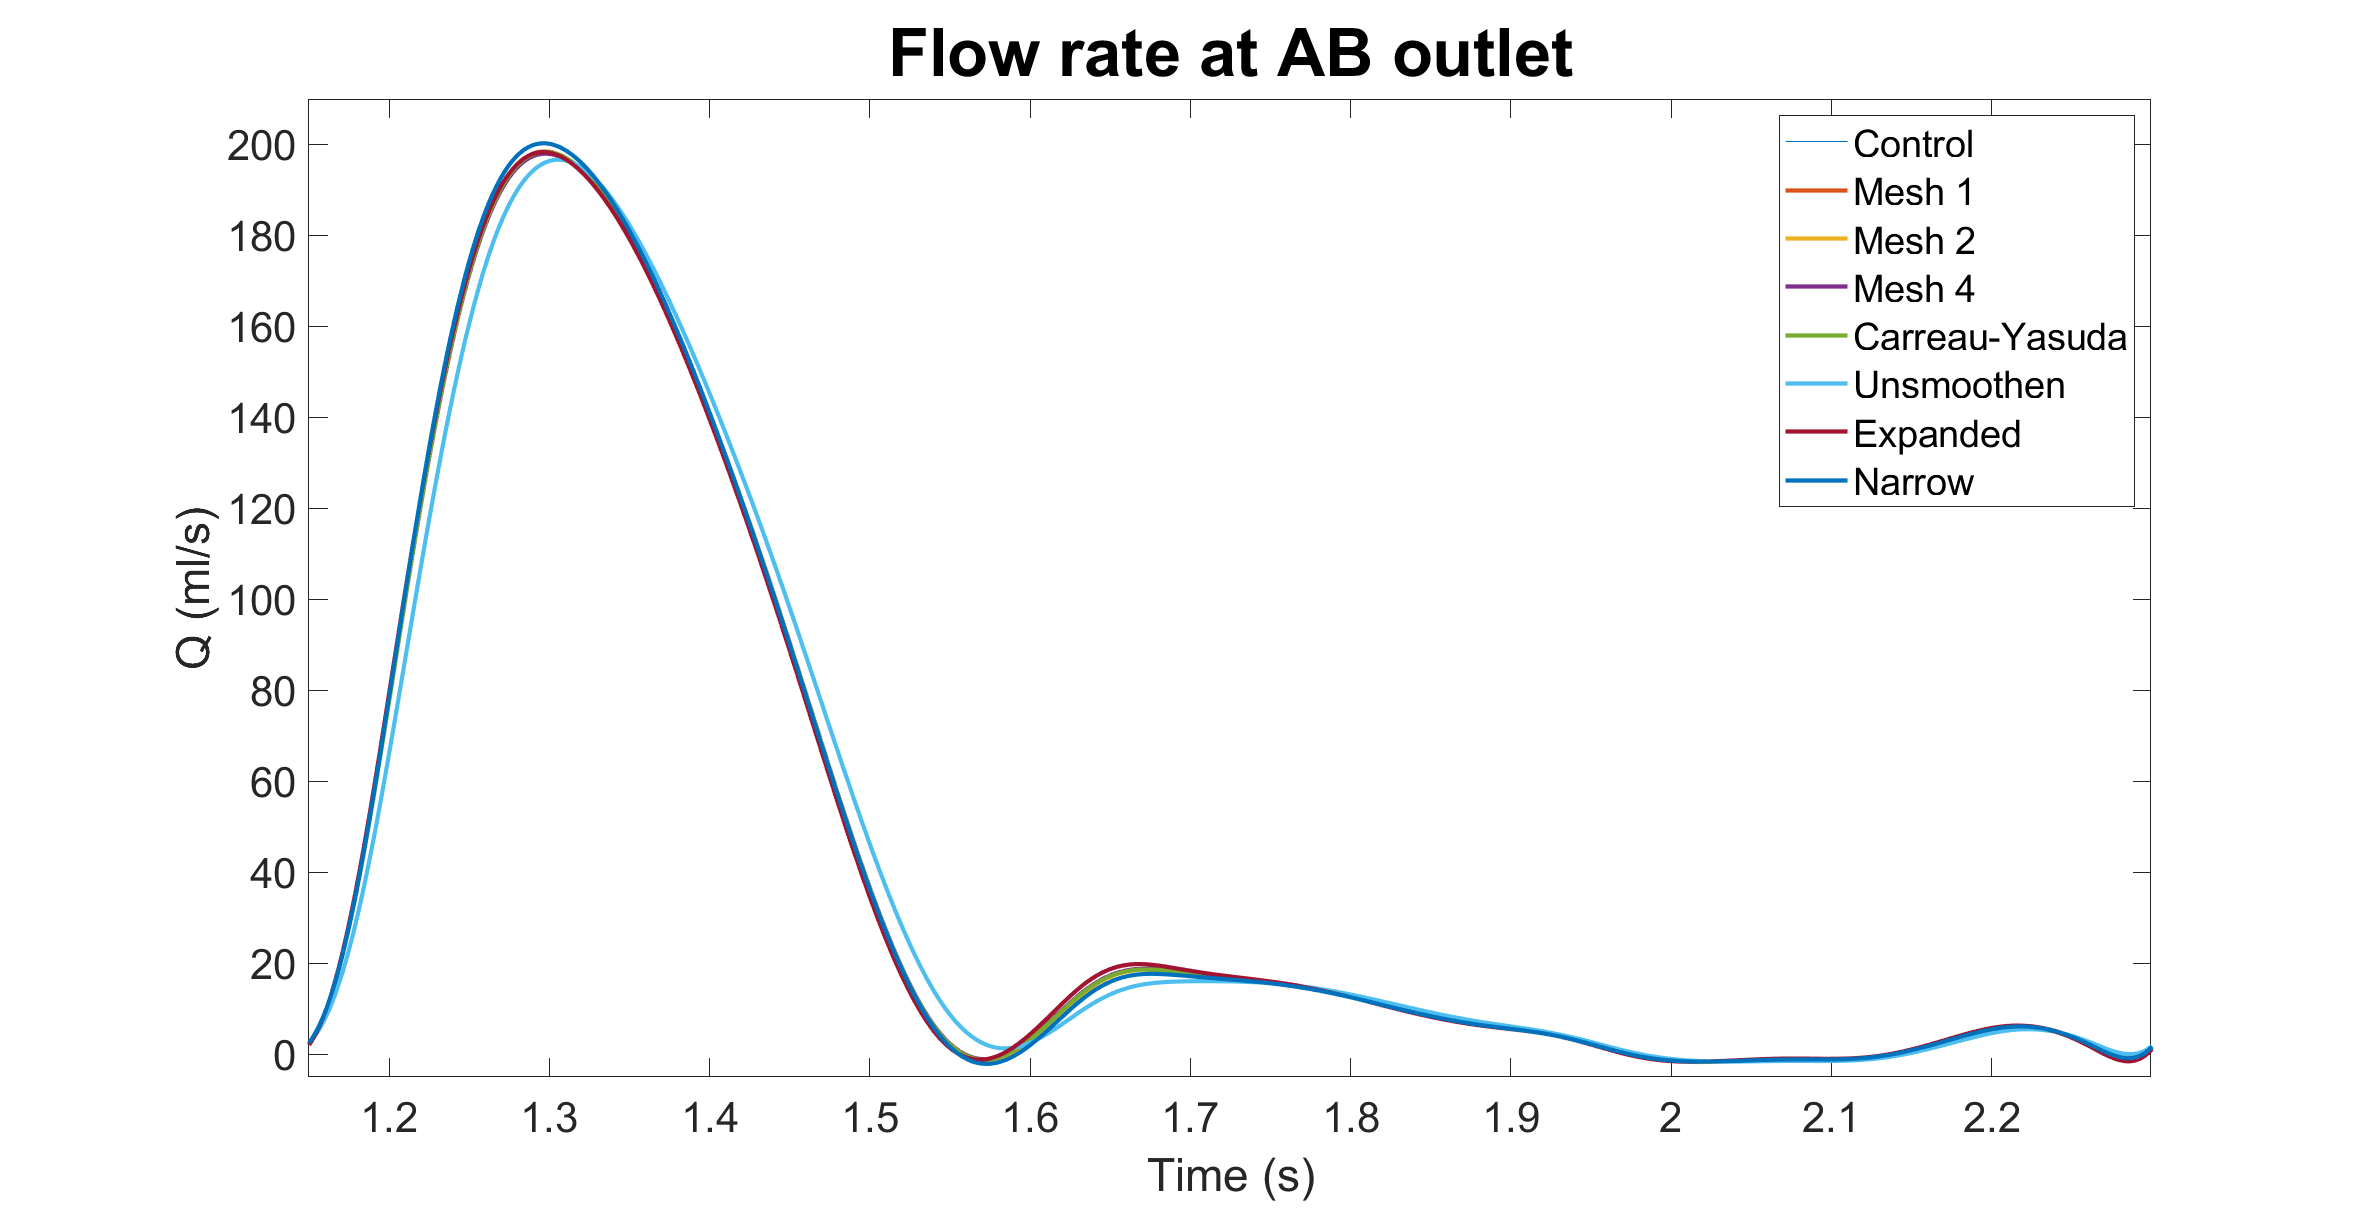
\includegraphics[width=\textwidth]{Figures/QAB.png}
     \end{subfigure}
     \hfill
     \begin{subfigure}[b]{0.49\textwidth}
         \centering
         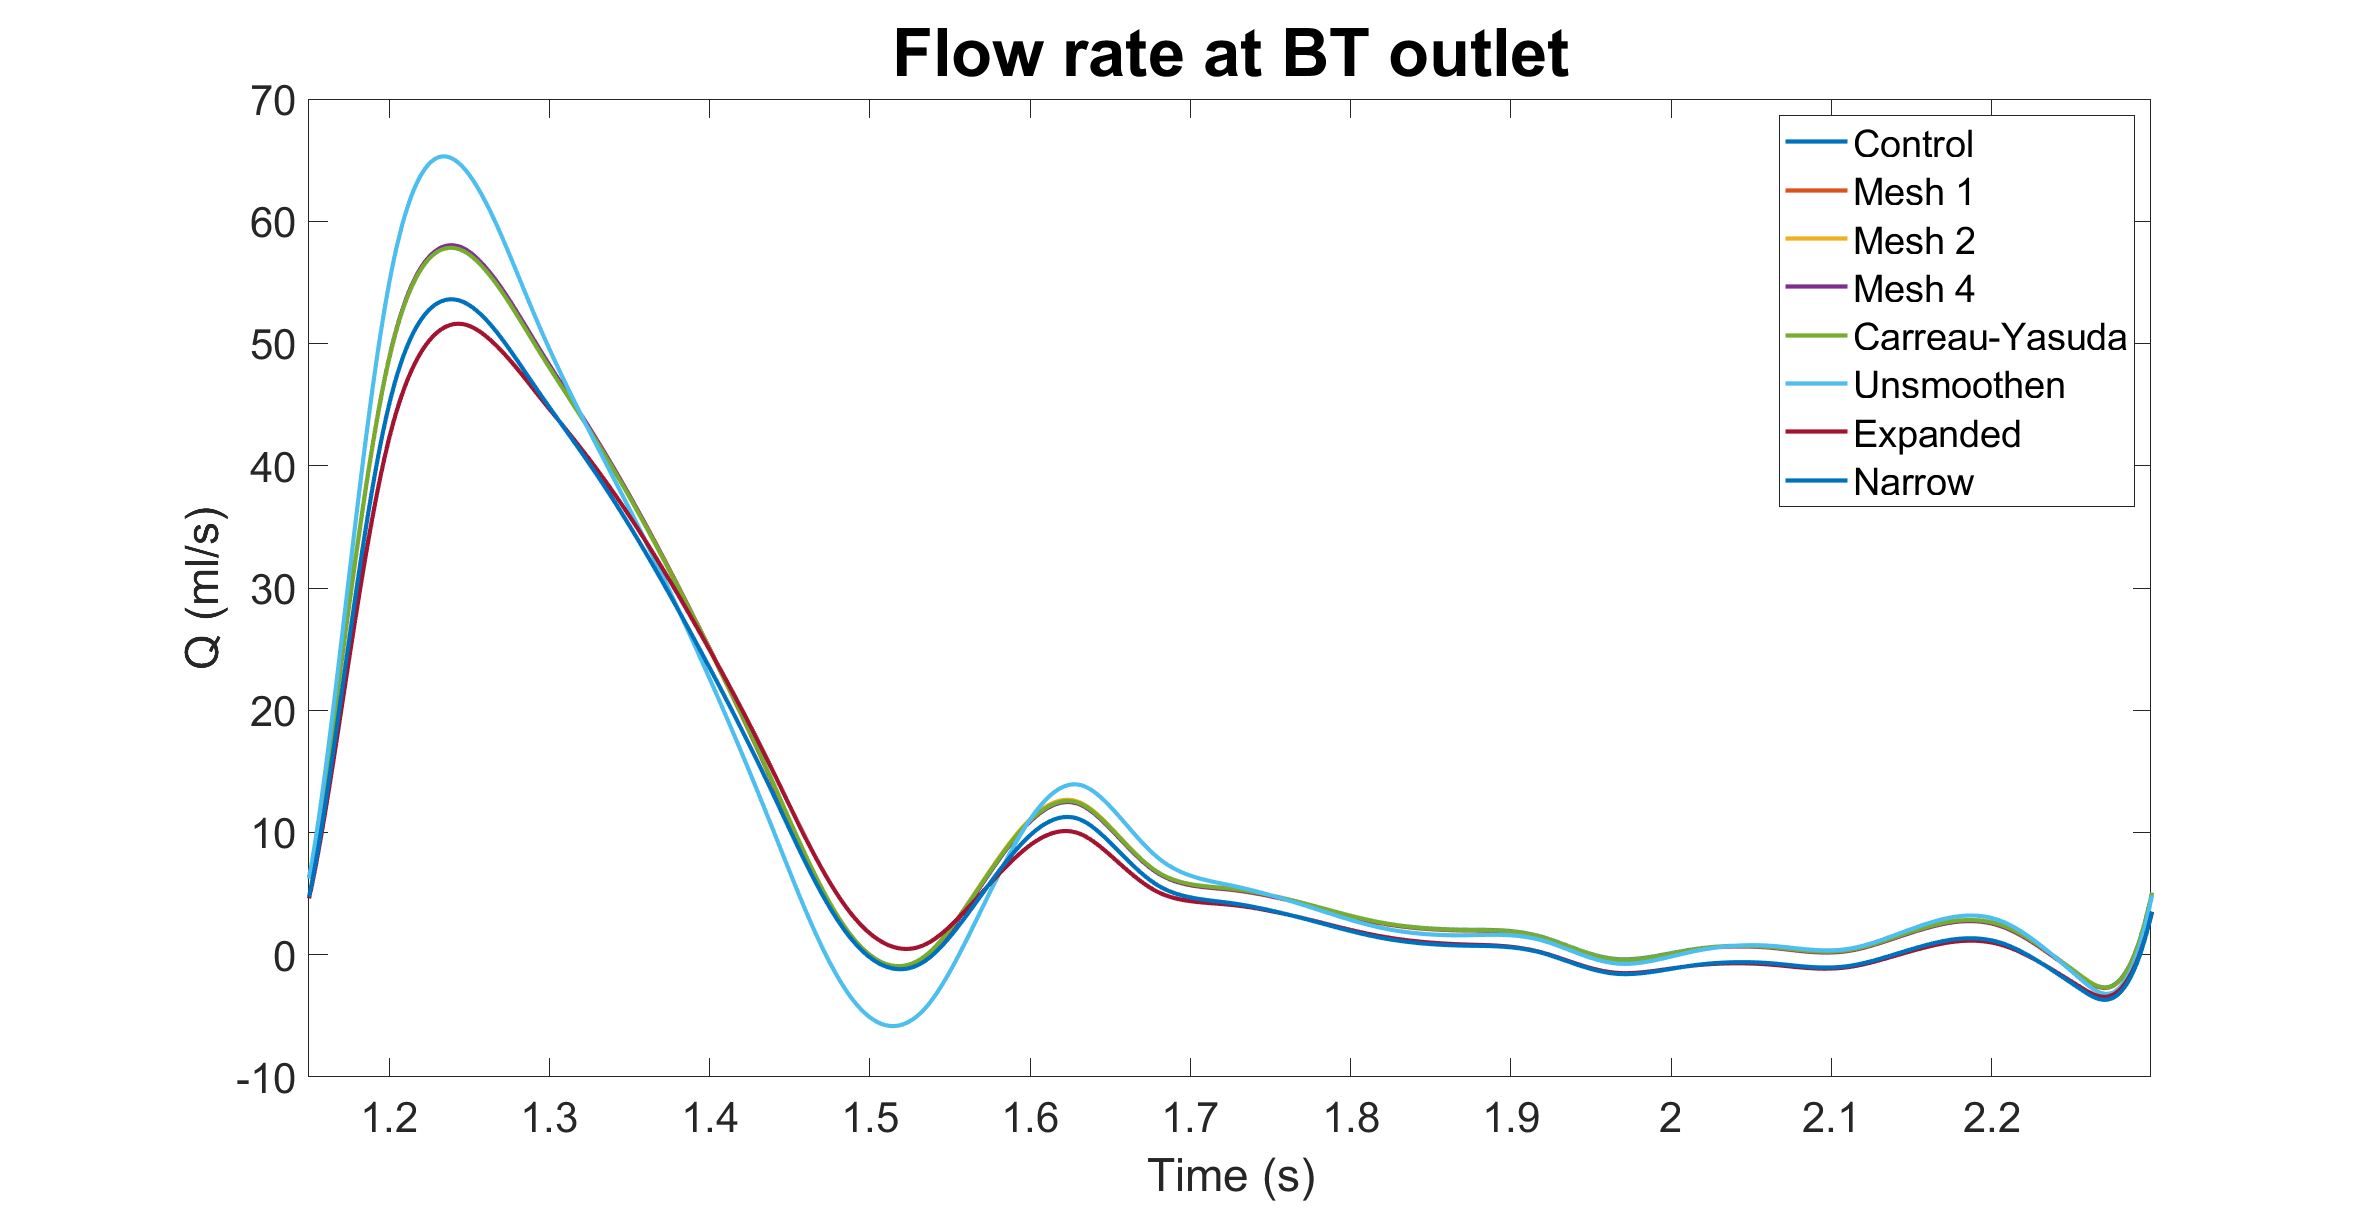
\includegraphics[width=\textwidth]{Figures/QBT.png}
     \end{subfigure}
     \hfill
     \begin{subfigure}[b]{0.49\textwidth}
         \centering
         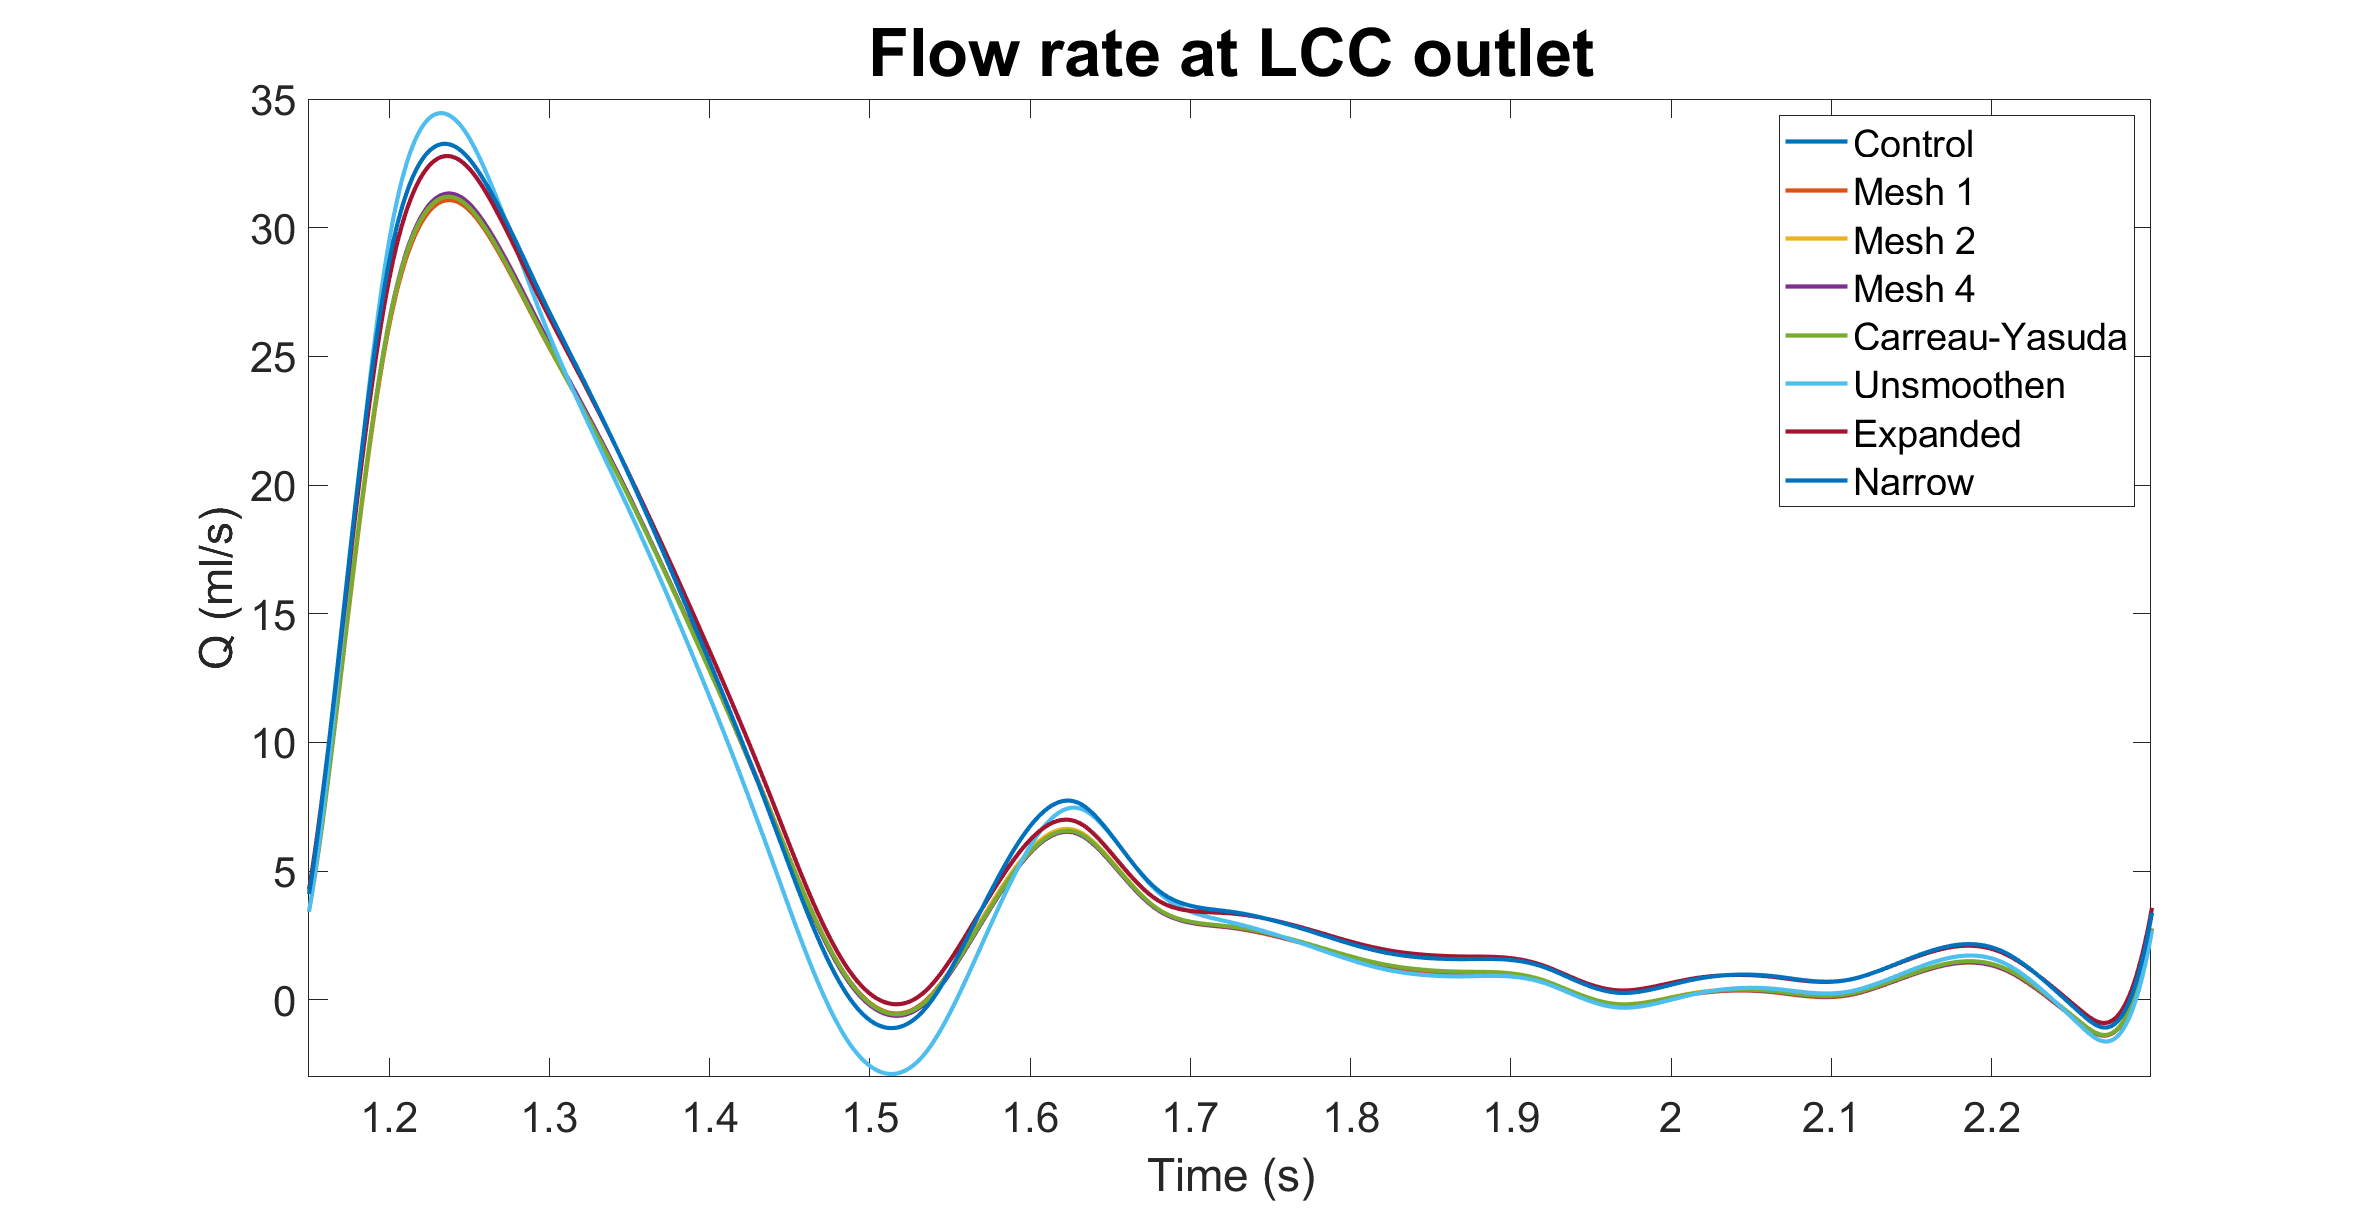
\includegraphics[width=\textwidth]{Figures/QLCC.png}
     \end{subfigure}
     \hfill
     \begin{subfigure}[b]{0.49\textwidth}
         \centering
         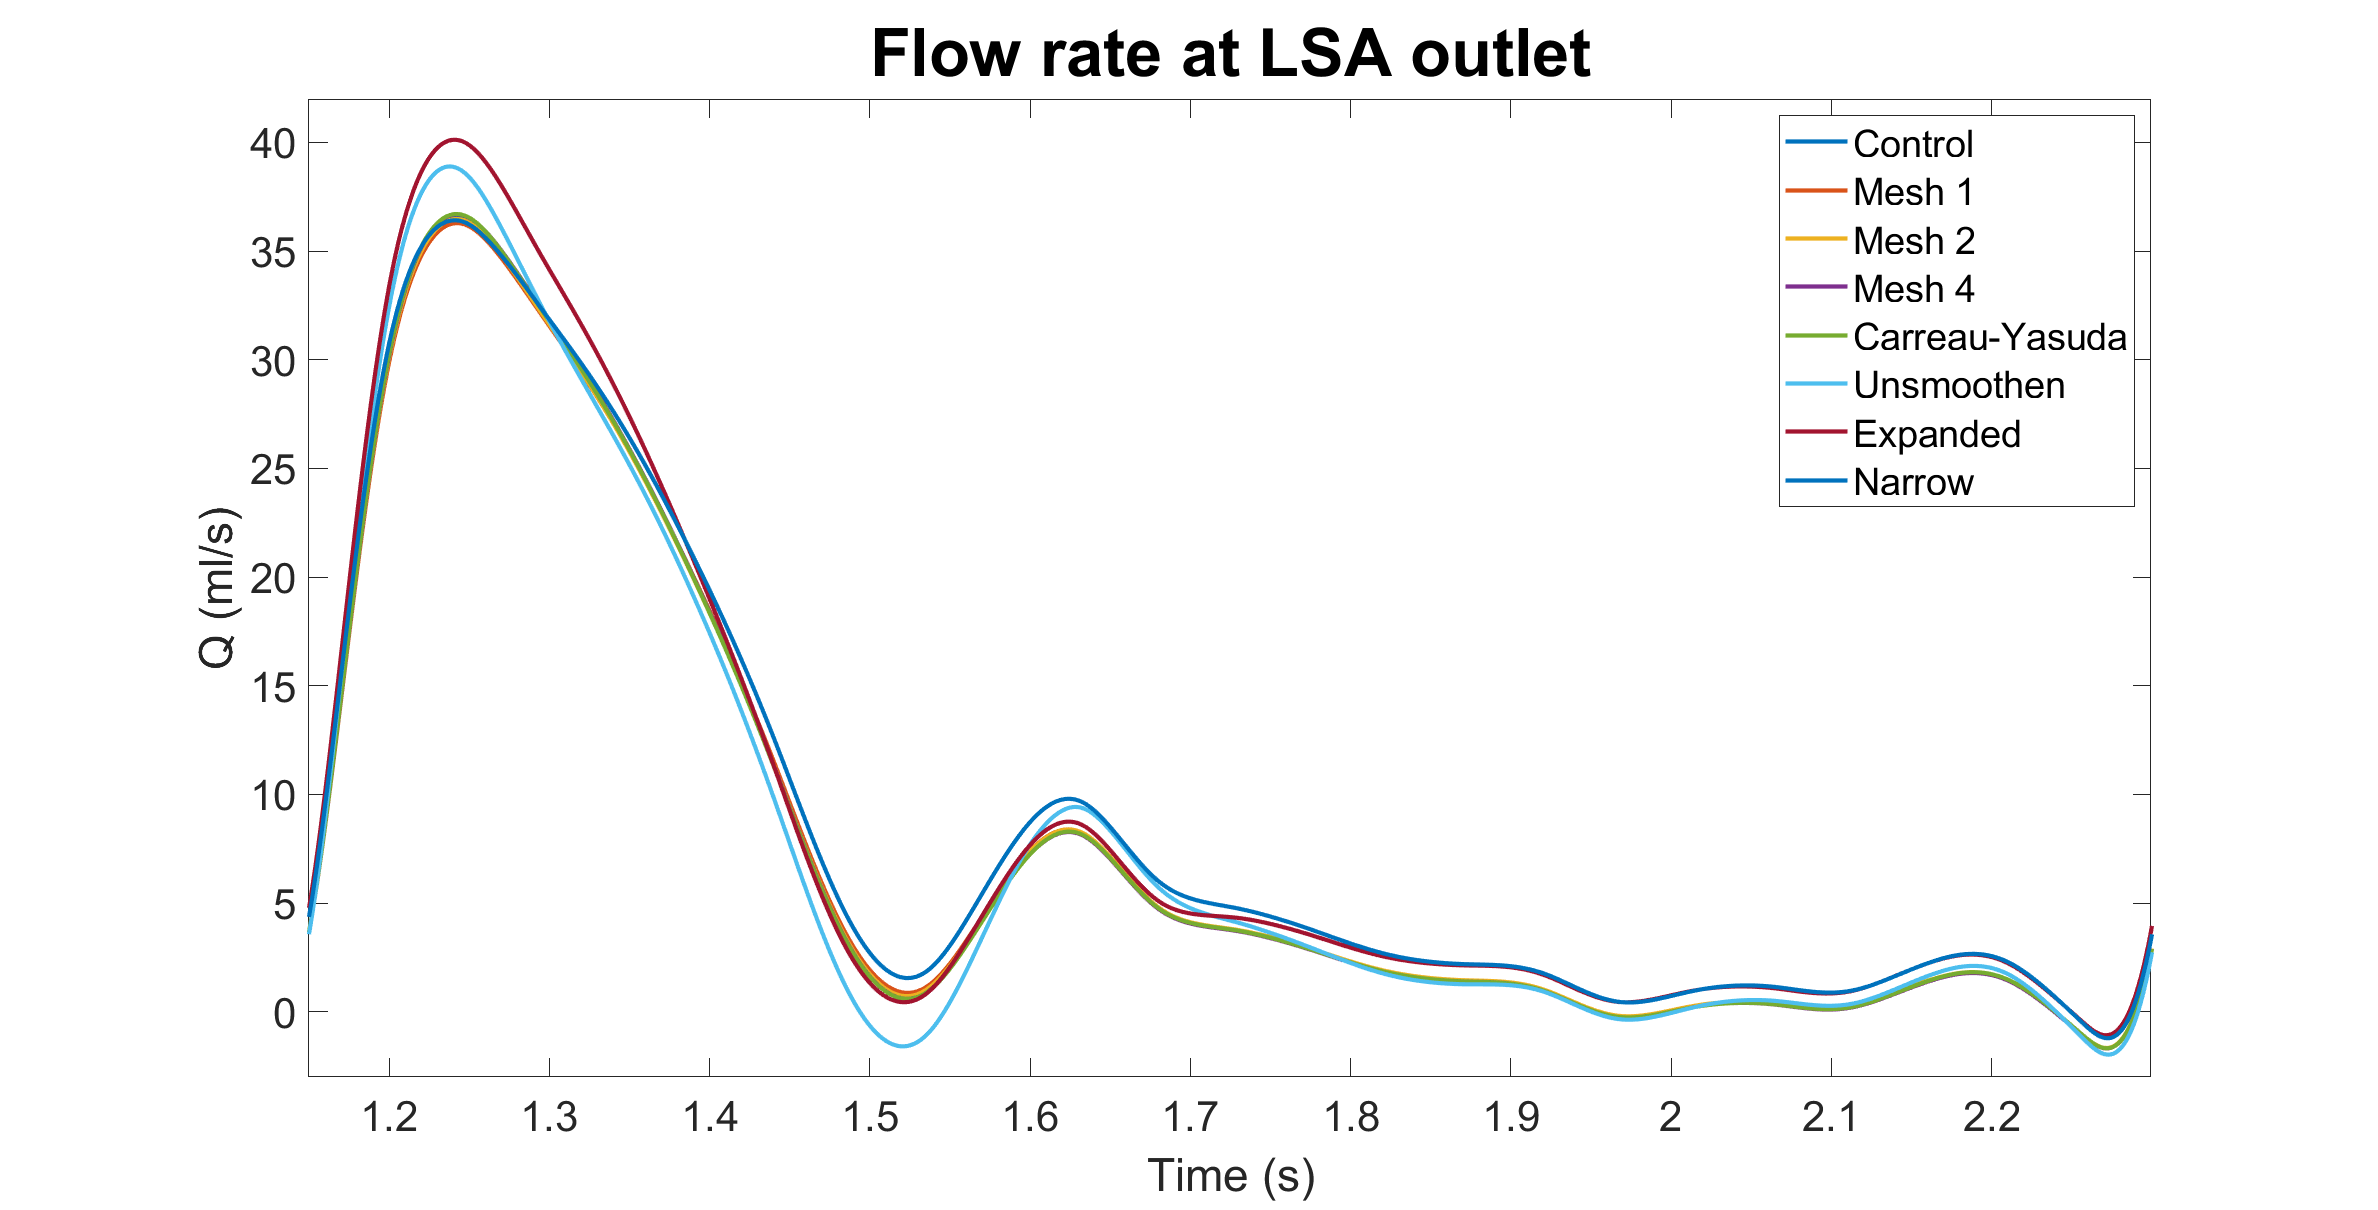
\includegraphics[width=\textwidth]{Figures/QLSA.png}
     \end{subfigure}
        \caption{The flow at the different outlets}
        \label{fig:flow}
\end{figure}

The most noticeable differences can be observed on the dilated geometries of the patient aorta, where the MAPE of the flow was up to  245.78\% at one of the outlet followed by the image processing influence, where the difference was 270.79\%. The smallest difference was shown to be the influence of the viscosity model, where the maximum MAPE is 6.24\%. The influence of the mesh showed varying results where the highest MAPE was calculated on the Mesh 1 with the maximum difference of 18.69\%. \par

\begin{table}[ht!]
\resizebox{\textwidth}{!}{%
\begin{tabular}{l|ccccccccc}
 & \multicolumn{9}{c}{Mean absolute percentage error (\%)} \\
Model & $P_{AB}$ & $P_{BT}$ & $P_{LCC}$ & $P_{LSA}$ & $P_{in}$ & $Q_{AB}$ & $Q_{BT}$ & $Q_{LCC}$ & $Q_{LSA}$ \\ \hline
Mesh 1 & 0.05 & 0.07 & 0.11 & 0.12 & 0.07 & 9.11 & 10.28 & 18.69 & 3.49 \\
Mesh 2 & 0.07 & 0.07 & 0.07 & 0.09 & 0.07 & 4.69 & 5.78 & 3.22 & 9.32 \\
Mesh 4 & 0.05 & 0.05 & 0.06 & 0.05 & 0.05 & 4.59 & 8.20 & 6.05 & 1.69 \\
Carreau-Yasuda & 0.03 & 0.04 & 0.04 & 0.04 & 0.06 & 3.11 & 6.24 & 4.27 & 3.63 \\
Unsmooth geometry & 0.51 & 0.85 & 0.76 & 0.53 & 1.00 & 71.36 & 270.79 & 138.30 & 36.97 \\
Expanded & 0.32 & 0.39 & 0.34 & 0.50 & 0.53 & 16.38 & 234.40 & 245.78 & 152.72 \\
Narrow & 0.52 & 0.56 & 0.35 & 0.69 & 0.77 & 18.40 & 180.13 & 224.91 & 159.92
\end{tabular}%
}
\caption{The mean absolute percentage error at the outlets between the different models and control}
\label{tab:pererr}
\end{table}

\section{Haemodynamic indices}
The results of TAWSS can be seen on the Table \ref{tab:meanTAWSS}. On the Figures \ref{fig:TAWSScontrol}-\ref{fig:TAWSSGeo1}, the aorta was divided in sections along the centerline and at every section, a box plot of haemodynamic indices was plotted. The box plot shows the mean of the values in the section with the red line, the $25^{th}$ and $75^{th}$ percentile of all the values and the maximum and the maximum the lines signify the maximum and minimum value. \par

\begin{table}[ht!]
\resizebox{\textwidth}{!}{%
\begin{tabular}{l|cccc}
 & \multicolumn{4}{c}{Mean TAWSS + SD at different locations (Pa)} \\
 & \multicolumn{1}{c|}{Ascending} & \multicolumn{1}{c|}{Arch} & \multicolumn{1}{c|}{Branches} & Descending \\ \hline
Control & \multicolumn{1}{c|}{0.996±0.630} & \multicolumn{1}{c|}{1.743±0.565} & \multicolumn{1}{c|}{1.979±0.893} & 1.152±0.388 \\
Mesh 1 & \multicolumn{1}{c|}{0.969±0.519} & \multicolumn{1}{c|}{1.714±0.543} & \multicolumn{1}{c|}{1.706±0.792} & 1.114±0.362 \\
Mesh 2 & \multicolumn{1}{c|}{0.986±0.562} & \multicolumn{1}{c|}{1.748±0.549} & \multicolumn{1}{c|}{1.832±0.829} & 1.154±0.390 \\
Mesh 4 & \multicolumn{1}{c|}{0.968±0.638} & \multicolumn{1}{c|}{1.708±0.556} & \multicolumn{1}{c|}{2.297±1.073} & 1.157±0.389 \\
CY & \multicolumn{1}{c|}{0.996±0.545} & \multicolumn{1}{c|}{1.633±0.478} & \multicolumn{1}{c|}{1.820±0.726} & 1.133±0.325 \\
Unsmooth geometry & \multicolumn{1}{c|}{1.357±0.798} & \multicolumn{1}{c|}{1.798±0.987} & \multicolumn{1}{c|}{2.468±1.522} & 1.757±0.852 \\
Expanded & \multicolumn{1}{c|}{0.938±0.545} & \multicolumn{1}{c|}{1.490±0.523} & \multicolumn{1}{c|}{1.498±0.700} & 1.007±0.341 \\
Narrow & \multicolumn{1}{c|}{1.151±0.719} & \multicolumn{1}{c|}{1.974±0.711} & \multicolumn{1}{c|}{2.598±1.592} & 1.302±0.514
\end{tabular}%
}
\caption{The mean TAWSS and the standard deviation (SD) of each model at different sections of the aorta}
\label{tab:meanTAWSS}
\end{table}

The most significant influence on the TAWSS can be seen on the model with the unsmooth geometry as a result of image processing where the mean TAWSS across all section is higher than the control model and the values of TAWSS have a wider spread as seen on the box plot (Figure \ref{fig:TAWSSImg}). \par

The expanded and narrow geometry results in a smaller and higher mean TAWSS respectively and it can be seen on the distribution of TAWSS (Figures \ref{fig:TAWSSGeo1} and \ref{fig:TAWSSGeo2}), however the shape of the TAWSS along the centerline seems to be similar to the one in the control model. The different mesh only shows small differences on the mean TAWSS values in the different sections and small changes can be seen on the distribution of TAWSS along the centerline (Figures \ref{fig:TAWSSMesh1}-\ref{fig:TAWSSMesh4}). Similar behaviour can be observed for the Carreau-Yasuda model (Figure \ref{fig:TAWSSVis}). \par

The 3D plots of TAWSS are shown in the Appendix \ref{appendix1}.

\begin{figure}[ht!]
    \centering
    \includegraphics[width=\textwidth]{"Figures/Control TAWSS".png}
    \caption{Control Model TAWSS box plot along centerline}
    \label{fig:TAWSScontrol}
\end{figure}
\begin{figure}[ht!]
    \centering
    \includegraphics[width=\textwidth]{"Figures/Mesh1 TAWSS".png}
    \caption{Mesh 1 Model TAWSS box plot along centerline}
    \label{fig:TAWSSMesh1}
\end{figure}
\begin{figure}[ht!]
    \centering
    \includegraphics[width=\textwidth]{"Figures/Mesh2 TAWSS".png}
    \caption{Mesh 2 Model TAWSS box plot along centerline}
    \label{fig:TAWSSMesh2}
\end{figure}
\begin{figure}[ht!]
    \centering
    \includegraphics[width=\textwidth]{"Figures/Mesh4 TAWSS".png}
    \caption{Mesh 4 Model TAWSS box plot along centerline}
    \label{fig:TAWSSMesh4}
\end{figure}
\begin{figure}[ht!]
    \centering
    \includegraphics[width=\textwidth]{"Figures/Viscosity TAWSS".png}
    \caption{Carreau-Yasuda Model TAWSS box plot along centerline}
    \label{fig:TAWSSVis}
\end{figure}
\begin{figure}[ht!]
    \centering
    \includegraphics[width=\textwidth]{"Figures/Img TAWSS".png}
    \caption{Unsmooth Geometry Model TAWSS box plot along centerline}
    \label{fig:TAWSSImg}
\end{figure}
\begin{figure}[ht!]
    \centering
    \includegraphics[width=\textwidth]{"Figures/Expanded TAWSS".png}
    \caption{Expanded lumen model TAWSS box plot along centerline}
    \label{fig:TAWSSGeo1}
\end{figure}
\begin{figure}[ht!]
    \centering
    \includegraphics[width=\textwidth]{"Figures/Narrow TAWSS".png}
    \caption{Narrow lumen model TAWSS box plot along centerline}
    \label{fig:TAWSSGeo2}
\end{figure}

\section{Interacting sources of variability}
Using the conceptual framework, additional models have been simulated which are used to assess the variability due to assumptions and identify the uncertain areas. Additionally, it is also possible for different assumptions to be interacting resulting in further uncertain error.\par

In order to show how the framework is used to generate additional models for the study of uncertainty, two more cases have been analysed. \par

\subsection{Segmentation-Viscosity model}
The effect of the segmentation geometry combined with the non-Newtonian viscosity is plotted on the Figure \ref{fig:TAWSSCYGeo1} and \ref{fig:TAWSSCYGeo2} and the mean TAWSS can be seen on the Table \ref{tab:meanCYTAWSS}. \par

A comparison with the corresponding Newtonian models shows that the mean TAWSS values due to the viscosity model are very similar. A similar trend can be seen in the comparison of the geometries. Based on these results, it can be seen that the blood viscosity model introduces very little variability to the results, while the segmentation can give significant variation.  

\begin{table}[ht!]
\resizebox{\textwidth}{!}{%
\begin{tabular}{l|cccc}
 & \multicolumn{4}{c}{Mean TAWSS + SD at different locations (Pa)} \\
 & \multicolumn{1}{c|}{Ascending} & \multicolumn{1}{c|}{Arch} & \multicolumn{1}{c|}{Branches} & Descending \\ \hline
Expanded CY &  \multicolumn{1}{c|}{0.949±0.554} & \multicolumn{1}{c|}{1.429±0.452} & \multicolumn{1}{c|}{1.431±0.588} & 1.012±0.291 \\
Narrow CY & \multicolumn{1}{c|}{1.131±0.617} & \multicolumn{1}{c|}{1.819±0.592} & \multicolumn{1}{c|}{2.319±1.254} & 1.260±0.424 \\
\end{tabular}%
}
\caption{The mean TAWSS and the standard deviation (SD) of segmentation and viscosity model}
\label{tab:meanCYTAWSS}
\end{table}

\begin{figure}[ht!]
    \centering
    \includegraphics[width=\textwidth]{"Figures/Expanded CY TAWSS".png}
    \caption{Expanded lumen Carreau-Yasuda model TAWSS box plot along centerline}
    \label{fig:TAWSSCYGeo1}
\end{figure}
\begin{figure}[ht!]
    \centering
    \includegraphics[width=\textwidth]{"Figures/Narrow CY TAWSS".png}
    \caption{Narrow lumen Carreau-Yasuda model TAWSS box plot along centerline}
    \label{fig:TAWSSCYGeo2}
\end{figure}


\subsection{Smoothing-Segmentation model}
Another case that has been analysed is the combined effect of the smoothing of the wall and the dilated geometries. \par

The TAWSS distribution along the centerline for both models are similar (Figures \ref{fig:TAWSSImgGeo1} \ref{fig:TAWSSImgGeo2}). In addition, the mean TAWSS at different sections are very similar as seen on Table \ref{tab:meanImgTAWSS}. \par

The comparison of the smooth and unsmooth geometry cases show different variability across the different sections of the aorta and in the mean values of TAWSS. Similarly the variation where the geometry is changed is different across models. This could be the result due to the interaction of the modelling choices, in this case, the dilation and the smoothing of the wall.

\begin{table}[ht!]
\centering
\resizebox{\textwidth}{!}{%
\begin{tabular}{l|cccc}
 & \multicolumn{4}{l}{Mean TAWSS + SD at different locations (Pa)} \\
 & Ascending & Arch & Branches & Descending \\ \hline
Unsmooth Geometry Expand & 1.287±0.800 & 1.693±0.947 & 1.861±1.122 & 1.532±0.744 \\
Unsmooth Geometry Narrow & 1.291±0.795 & 1.732±0.976 & 1.853±1.119 & 1.532±0.744
\end{tabular}%
}
\caption{The mean TAWSS and the standard deviation (SD) of segmentation and smoothing}
\label{tab:meanImgTAWSS}
\end{table}

\begin{figure}[ht!]
    \centering
    \includegraphics[width=\textwidth]{"Figures/Unsmooth Expanded TAWSS".png}
    \caption{Unsmooth Geometry Expanded lumen model TAWSS box plot along centerline}
    \label{fig:TAWSSImgGeo1}
\end{figure}
\begin{figure}[ht!]
    \centering
    \includegraphics[width=\textwidth]{"Figures/Unsmooth Narrow TAWSS".png}
    \caption{Unsmooth Geometry Narrow lumen model TAWSS box plot along centerline}
    \label{fig:TAWSSImgGeo2}
\end{figure}
